%%**************************************************************
%% Vorlage DHBW Arbeiten
%%
%% Autor: Carl, Winkler
%% Datum: 01.05.2018
%%
%%**************************************************************
\documentclass[%
	pdftex,
	oneside,		% Einseitiger Druck.
	12pt,			% Schriftgroesse
	parskip=half,	% Halbe Zeile Abstand zwischen Absätzen.
	headsepline,	% Linie nach Kopfzeile.
	footsepline,	% Linie vor Fusszeile.
	abstracton,	    % Abstract Überschriften
	ngerman,		% Translator
]{scrreprt}
%!TEX root = ../dokumentation.tex



%svg
\usepackage{svg}

%Zoltan namensproblem
\usepackage[utf8]{inputenc} \usepackage[T1]{fontenc} 
\usepackage{lmodern} 

%Seitengroesse
\usepackage{fullpage}

%Tikz

\usepackage{amsmath}
\usepackage{tikz}
\usepackage{mathdots}
\usepackage{yhmath}
\usepackage{cancel}
\usepackage{color}

%Zeilenumbruch und mehr
\usepackage[activate]{microtype}

% Zeichencodierung
\usepackage[utf8]{inputenc}
\usepackage[T1]{fontenc}

% Zeilenabstand
\usepackage[onehalfspacing]{setspace}

% Index-Erstellung
\usepackage{makeidx}

% Tabellen
\usepackage{booktabs}

% Lokalisierung (neue deutsche Rechtschreibung)
\usepackage[ngerman]{babel}

% Anführungszeichen 
\usepackage[babel,german=quotes]{csquotes}
%\usepackage[style=swiss]{csquotes}


% Spezielle Tabellenform fuer Deckblatt
\usepackage{longtable}
\setlength{\tabcolsep}{10pt} %Abstand zwischen Spalten
\renewcommand{\arraystretch}{1.5} %Zeilenabstand

% Grafiken
\usepackage{graphicx}

% Mathematische Textsaetze
%\usepackage{amsmath}
%\usepackage{amssymb}

% Pakete um Textteile drehen zu können, oder eine Seite Querformat anzeigen kann.
%\usepackage{rotating}
%\usepackage{lscape}

% Farben
\usepackage{color}
\definecolor{LinkColor}{rgb}{0,0,0.2}
\definecolor{ListingBackground}{rgb}{0.92,0.92,0.92}

\newcommand{\pdftitel}{Verhaltenssteuerung eines autonomen Fahrzeugs mit Zustandsautomaten}
\newcommand{\autor}{Carl Fabian Winkler}
\newcommand{\arbeit}{T3100 Studienarbeit}

% Titel, Autor und Datum
\title{\titel}
\author{\autor}
\date{\datum}

% PDF Einstellungen
\usepackage[%
	pdftitle={\pdftitel},
	pdfauthor={\autor},
	pdfsubject={\arbeit},
	pdfcreator={pdflatex, LaTeX with KOMA-Script},
	pdfpagemode=UseOutlines, % Beim Oeffnen Inhaltsverzeichnis anzeigen
	pdfdisplaydoctitle=true, % Dokumenttitel statt Dateiname anzeigen.
	pdflang=de % Sprache des Dokuments.
]{hyperref} 

% (Farb-)einstellungen für die Links im PDF
\hypersetup{%
	colorlinks=true, % Aktivieren von farbigen Links im Dokument
	linkcolor=LinkColor, % Farbe festlegen
	citecolor=LinkColor,
	filecolor=LinkColor,
	menucolor=LinkColor,
	urlcolor=LinkColor,
	bookmarksnumbered=true % Überschriftsnummerierung im PDF Inhalt anzeigen.
}

% Literaturverweise nach Harvard (mit deutschem und)
%\usepackage[dcucite]{harvard}
%\renewcommand{\harvardand}{und}
\usepackage[
backend=biber,
style=alphabetic,
sorting=ynt
]{biblatex}
\addbibresource{ArbeitBib.bib}
% Verschiedene Schriftarten
%\usepackage{goudysans}
%\usepackage{lmodern}
%\usepackage{libertine}
\usepackage{helvet} 
\renewcommand{\rmdefault}{phv}
%\renewcommand{\sfdefault}{phv}
%\renewcommand{\mddefault}{b}
%\renewcommand{\bfdefault}{b} % Helvetica has no bx series
%\renewcommand{\updefault}{sl}
% Hurenkinder und Schusterjungen verhindern
% http://projekte.dante.de/DanteFAQ/Silbentrennung
\clubpenalty=10000
\widowpenalty=10000
\displaywidowpenalty=10000
%Tables
\usepackage{makecell}
% Quellcode
\usepackage{listings}
\lstloadlanguages{Java}
\lstset{%
	language=PHP,		 	 % Sprache des Quellcodes
	%numbers=left,           % Zelennummern links
	stepnumber=1,            % Jede Zeile nummerieren.
	numbersep=5pt,           % 5pt Abstand zum Quellcode
	numberstyle=\tiny,       % Zeichengrösse 'tiny' für die Nummern.
	breaklines=true,         % Zeilen umbrechen wenn notwendig.
	breakautoindent=true,    % Nach dem Zeilenumbruch Zeile einrücken.
	postbreak=\space,        % Bei Leerzeichen umbrechen.
	tabsize=2,               % Tabulatorgrösse 2
	basicstyle=\ttfamily\footnotesize, % Nichtproportionale Schrift, klein für den Quellcode
	showspaces=false,        % Leerzeichen nicht anzeigen.
	showstringspaces=false,  % Leerzeichen auch in Strings ('') nicht anzeigen.
	extendedchars=true,      % Alle Zeichen vom Latin1 Zeichensatz anzeigen.
	captionpos=b,            % sets the caption-position to bottom
	backgroundcolor=\color{ListingBackground} % Hintergrundfarbe des Quellcodes setzen.
}
\usepackage{caption}
\usepackage{varwidth}
\DeclareCaptionFormat{myformat}{%
  % #1: label (e.g. "Table 1")
  % #2: separator (e.g. ": ")
  % #3: caption text
  \begin{varwidth}{\linewidth}%
    \centering
    #1#2#3%
  \end{varwidth}%
}
%\usepackage{subcaption}
% Glossar
\usepackage[
	nonumberlist, %keine Seitenzahlen anzeigen
	%acronym,      %ein Abkürzungsverzeichnis erstellen
	%section,     %im Inhaltsverzeichnis auf section-Ebene erscheinen
	toc,          %Einträge im Inhaltsverzeichnis
]{glossaries}

%Akronyme
\usepackage{acronym}
%\usepackage{acro}[2015/02/26]
% Fussnoten
\usepackage[perpage, hang, multiple, stable]{footmisc}

%Bildpfad
\graphicspath{{images/}}

%nur ein latex-Durchlauf für die Aktualisierung von Verzeichnissen nötig
\usepackage{bookmark}

%Gleitumgebungen (Bilder, Tabellen, usw\ldots) lassen sich mit H an genau der
% definierten Stelle platzieren
\usepackage{float}

% für die vertikale Platzierung von Text in Tabellen
\usepackage{array}

% für die Darstellung des Euro-Symbols
\usepackage[right]{eurosym}

% für textumflossene Grafiken
\usepackage{wrapfig}

% eine Kommentarumgebung "k" (Handhabe mit \begin{k}<Kommentartext>\end{k},
% Kommentare werden rot gedruckt). Wird \% vor excludecomment{k} entfernt,
% werden keine Kommentare mehr gedruckt.
\usepackage{comment}
\specialcomment{k}{\begingroup\color{red}}{\endgroup}

%counter für Abbildungen
\usepackage{chngcntr}
\counterwithout{figure}{chapter}

%Ohm Zeichen
\usepackage{siunitx}

\usepackage{dirtree}
%\excludecomment{k}

%Barriere
\usepackage[section]{placeins}

% Ab jetzt können auch Umlaute verwendet werden

%falls pdftitel = titel der Arbeit
\newcommand{\titel}{\pdftitel}
%bei unterschiedlichen Titeln
%\newcommand{\titel}{l haben wir einen zweizeiligen
% Bachelorthesistitel}
\newcommand{\martrikelnr}{1695079}
\newcommand{\kurs}{ITA17}
\newcommand{\datumAbgabe}{8. Juni 2020}
\newcommand{\firma}{Magna PT B.V. \& Co. KG}
\newcommand{\firmenort}{Untergruppenbach}
\newcommand{\abgabeort}{Stuttgart}
\newcommand{\abschluss}{Bachelor of Science}
\newcommand{\studiengang}{IT Automotive}
\newcommand{\dhbw}{Stuttgart}
\newcommand{\betreuer}{Prof. Dr. Zoltan Adam Zomotor}
\newcommand{\gutachter}{Dr. Who}
\newcommand{\zeitraum}{20.01.2020 - 08.06.2020}
\newcommand{\arbeitsart}{\arbeit}
\renewcommand*{\chapterheadstartvskip}{\vspace*{1cm}}

\makeglossaries
%!TEX root = ../dokumentation.tex

%
% vorher in Konsole folgendes aufrufen: 
%	makeglossaries makeglossaries dokumentation.acn && makeglossaries dokumentation.glo
%

%
% Glossareintraege --> referenz, name, beschreibung
% Aufruf mit \gls{...}
%
\newglossaryentry{Glossareintrag}{name={Glossareintrag},plural={Glossareinträge},description={Ein Glossar beschreibt verschiedenste Dinge in kurzen Worten}}


\begin{document}

	% Deckblatt
	\begin{spacing}{1}
		%!TEX root = ../dokumentation.tex

\begin{titlepage}
%\setlength\LTleft{0pt}
%\setlength\LTright{0pt}
    \begin{figure}
\centering
\begin{minipage}{.4\textwidth}
    %\includesvg[height=1.2cm]{images/Magna_logo.svg}
\end{minipage}%
\begin{minipage}{.4\textwidth}
    \begin{flushright}
    \includesvg[height=2.4cm]{images/DHBW_Logo.svg}
    \end{flushright}
\end{minipage}
\end{figure}
	%\begin{longtable}{lr}
	  %{\includesvg[height=1.2cm]{images/Magna_logo.svg}} & 
	  %{\includesvg[height=1.2cm]{images/DHBW_Logo.svg}}
	%\end{longtable}
	\enlargethispage{20mm}
	\begin{center}
	  \vspace*{12mm}	{\large\textbf \titel }\\
	  \vspace*{12mm}	{\large\textbf \arbeit}\\
	  
	  \vspace*{12mm}	\studiengang\\
	  \vspace*{3mm} 	an der Dualen Hochschule Baden-Württemberg \dhbw\\
	  \vspace*{12mm}	von\\
	  \vspace*{3mm} 	{\large\textbf \autor}\\
	  \vspace*{12mm}	\datumAbgabe\\
	\end{center}
	\vfill
	\begin{spacing}{1.2}
	\begin{tabbing}
		mmmmmmmmmmmmmmmmmmmmmmmmmm     \= \kill
		\textbf{Bearbeitungszeitraum}  \>  \zeitraum\\
		\textbf{Matrikelnummer, Kurs}  \>  \martrikelnr, \kurs\\
		%\textbf{Ausbildungsfirma}      \>  \firma, \firmenort\\
		\textbf{Betreuer}              \>  \betreuer\\
		%\textbf{Gutachter}             \>  \gutachter
	\end{tabbing}
	\end{spacing}
\end{titlepage}

	\end{spacing}
	\newpage

	\renewcommand{\thepage}{\Roman{page}}
	\setcounter{page}{1}

	% Sperrvermerk
	% \cleardoublepage
	% %!TEX root = ../dokumentation.tex

%\thispagestyle{empty}
% Sperrvermerk direkt hinter Titelseite
\section*{Sperrvermerk}
\addcontentsline{toc}{chapter}{Sperrvermerk}

\vspace*{2em}

Die vorliegende {\arbeitsart} mit dem Titel {\itshape \titel} ist mit einem Sperrvermerk versehen und wird ausschließlich zu Prüfungszwecken am Studiengang {\studiengang} der Dualen Hochschule Baden-Württemberg {\abgabeort} vorgelegt.
Jede Einsichtnahme und Veröffentlichung, auch von Teilen der Arbeit, bedarf der vorherigen Zustimmung durch die Firma {\firma}.


	% \newpage
	
	% Erklärung
	\cleardoublepage
	%!TEX root = ../dokumentation.tex

%\thispagestyle{empty}

%\section*{Erklärung}
\addcontentsline{toc}{chapter}{Erklärung}
% http://www.se.dhbw-mannheim.de/fileadmin/ms/wi/dl_swm/dhbw-ma-wi-organisation-bewertung-bachelorarbeit-v2-00.pdf
\vspace*{2em}


\noindent\fbox{%
    \parbox{\textwidth}{%
    \vspace*{1em}
    \FloatBarrier
    \centerline{\textit{Erklärung}}
    \FloatBarrier
    \vspace*{1em}
Ich versichere hiermit, dass ich meine Studienarbeit mit dem Thema: {\itshape \titel } selbstständig verfasst und keine anderen als die angegebenen Quellen und Hilfsmittel
benutzt habe.\par
Ich versichere zudem, dass die eingereichte elektronische Fassung mit der gedruckten Fassung
übereinstimmt.
\vspace*{3em}
\FloatBarrier
 - - - - - - - - - - - - - - - - - - - -                    \par
\textit{Ort}\hspace{2cm}\textit{Datum}\hspace{5cm}\textit{Unterschrift}
\vspace*{1em}
}
}

	\newpage

	% Abstract
	\cleardoublepage
	%!TEX root = ../dokumentation.tex

%\pagestyle{empty}

%\renewcommand{\abstractname}{Abstract}
%\begin{abstract}

%\end{abstract}

\chapter*{Zusammenfassung}
\addcontentsline{toc}{chapter}{Zusammenfassung}
Die vorliegende Arbeit beschreibt, wie die Softwarestruktur für ein autonomes Modellfahrzeug zur Teilnahme am Carolocup 2020 aufgebaut werden soll. Ziel der Arbeit ist es, die Verhaltenssteuerung für dieses autonome Fahrzeug zu entwerfen. Die Software wird auf dem Rechner des Fahrzeugs implementiert und getestet. Dabei wird insbesondere die Wartbarkeit und Erweiterbarkeit der Software berücksichtigt. Es wird zudem ermöglicht, den aktuellen Zustand des Fahrzeugs über einen Monitor einzusehen und Messwerte zu exportieren. Das Fahrzeug soll einen Parcour autonom befahren. Dabei müssen unter anderem Hindernisse überholt werden, fehlende Spuren erkannt und Vorfahrtsituationen an Kreuzungen beachtet werden.
\chapter*{Abstract}

\addcontentsline{toc}{chapter}{Abstract}

	\newpage

	\pagestyle{plain}

	% Inhaltsverzeichnis
	\begin{spacing}{1.1}
		\setcounter{tocdepth}{2}
		%für die Anzeige von Unterkapiteln im Inhaltsverzeichnis
		%\setcounter{tocdepth}{2}
		\tableofcontents
	\end{spacing}
	\newpage
	
	% Abkürzungsverzeichnis
    \cleardoublepage
	\phantomsection \label{listofacs}
    \addcontentsline{toc}{chapter}{Abkürzungsverzeichnis}
	%!TEX root = ../dokumentation.tex

\chapter*{Abkürzungsverzeichnis}
%nur verwendete Akronyme werden letztlich im Dokument angezeigt
\begin{acronym}[YTMMM]

\setlength{\itemsep}{-\parsep}
\acro{ROS}{Robot Operating System, Betriebssystem für autonome Systeme}
\acro{DHBW}{Duale Hochschule Baden Württemberg}
\end{acronym}


	% Abbildungsverzeichnis
	\cleardoublepage
	\phantomsection \label{listoffig}
	\addcontentsline{toc}{chapter}{Abbildungsverzeichnis}
	\listoffigures
	
	
	%Tabellenverzeichnis
	\cleardoublepage
	\phantomsection \label{listofftab}
	\addcontentsline{toc}{chapter}{Tabellenverzeichnis}
	\listoftables
	\clearpage
	
	\renewcommand{\thepage}{\arabic{page}}
	\setcounter{page}{1}
	
	% Inhalt
	%!TEX root = ../dokumentation.tex

\chapter{Einleitung}
\section{Motivation}
In der heutigen Zeit sind Fahrzeuge mit diversen Fahrerassistenzsystemen  zur Teilautomatisierung des Fahrens bereits auf dem Markt etabliert. Viele Fahrzeuge können automatisch einparken oder die Spur unter bestimmten Bedingungen halten. Der Trend bewegt sich seit Jahren von der Teilautomatisierung bestimmter Funktionen dazu immer mehr Funktionen zu automatisieren. Ein besonderer Meilenstein in dieser Entwicklung konnte bereits 2007 durch die DARPA Urban Challenge erreicht werden. Hier zeigten verschiedene Forscherteams die Machbarkeit von autonomen Fahrzeugen. Das autonome Fahren verspricht Komfortgewinn aber auch Kosteneinsparungen durch das Wegfallen von bezahlten Fahrern und erhöhte Sicherheit. Im Jahr 2018 starb laut Statistischem Bundesamt \cite{STA18} 3180 Menschen in Verkehrsunfällen. Über 300.000 Menschen wurden verletzt. Von den erfassten Unfällen lassen sich 88\% auf menschliches Fehlverhalten zurückführen.
Somit wird erwartet, dass diese Zahlen mit Durchsetzung des autonomen Fahrens drastisch zurückgehen werden. Daher forschen im Moment zahlreiche Universitäten, Fahrzeughersteller und Zulieferer an der Umsetzung des autonomen Fahren. Die Herausforderung dabei ist insbesondere der Entwurf geeigneter Softwarestrukturen und die sichere Implementierung einzelner Module für diese Systeme.

\section{Carolo-Cup Wettbewerb}
Der Carolo-Cup ist ein Hochschulwettbewerb an der Technischen Universität Braunschweig. Das Ziel des Carolo-Cups ist es, dass sich Studentierdenteams  mit der Entwicklung und Umsetzung von autonomen Modellfahrzeugen beschäftigen.

Die Modellfahrzeuge werden in unterschiedlichen realitätsnahen Szenarien miteinander verglichen und bewertet. Im Basic-Cup, der Anfängerklasse des Wettbewerbs, müssen zwei Strecken von den Modellfahrzeugen befahren werden. Eine dieser Strecken ist in Abbildung \ref{EIN:FOT} zu sehen. Im \"Obstacle Evasion\" Kurs müssen die autonomen Fahrzeuge stehende und bewegliche Hindernisse überholen. Im "Free Drive" Kurs muss das Fahrzeug möglichst viele Meter Strecke fahren. Auf beiden Strecken sollte das Fahrzeug zwei Mal autonom an einem dafür markierten Abschnitt der Strecke einparken. Zudem stellen die Teams als Teil des Wettbewerbs die erarbeiteten Konzepte einer Fachjury aus Wirtschaft und Wissenschaft vor. Dabei werden neben der Schlüssigkeit des Gesamtkonzeptes Aspekte wie Projektmanagement, Energie- und Kosteneffizienz bewertet. 
\FloatBarrier
\begin{figure}[h]
  \centering
  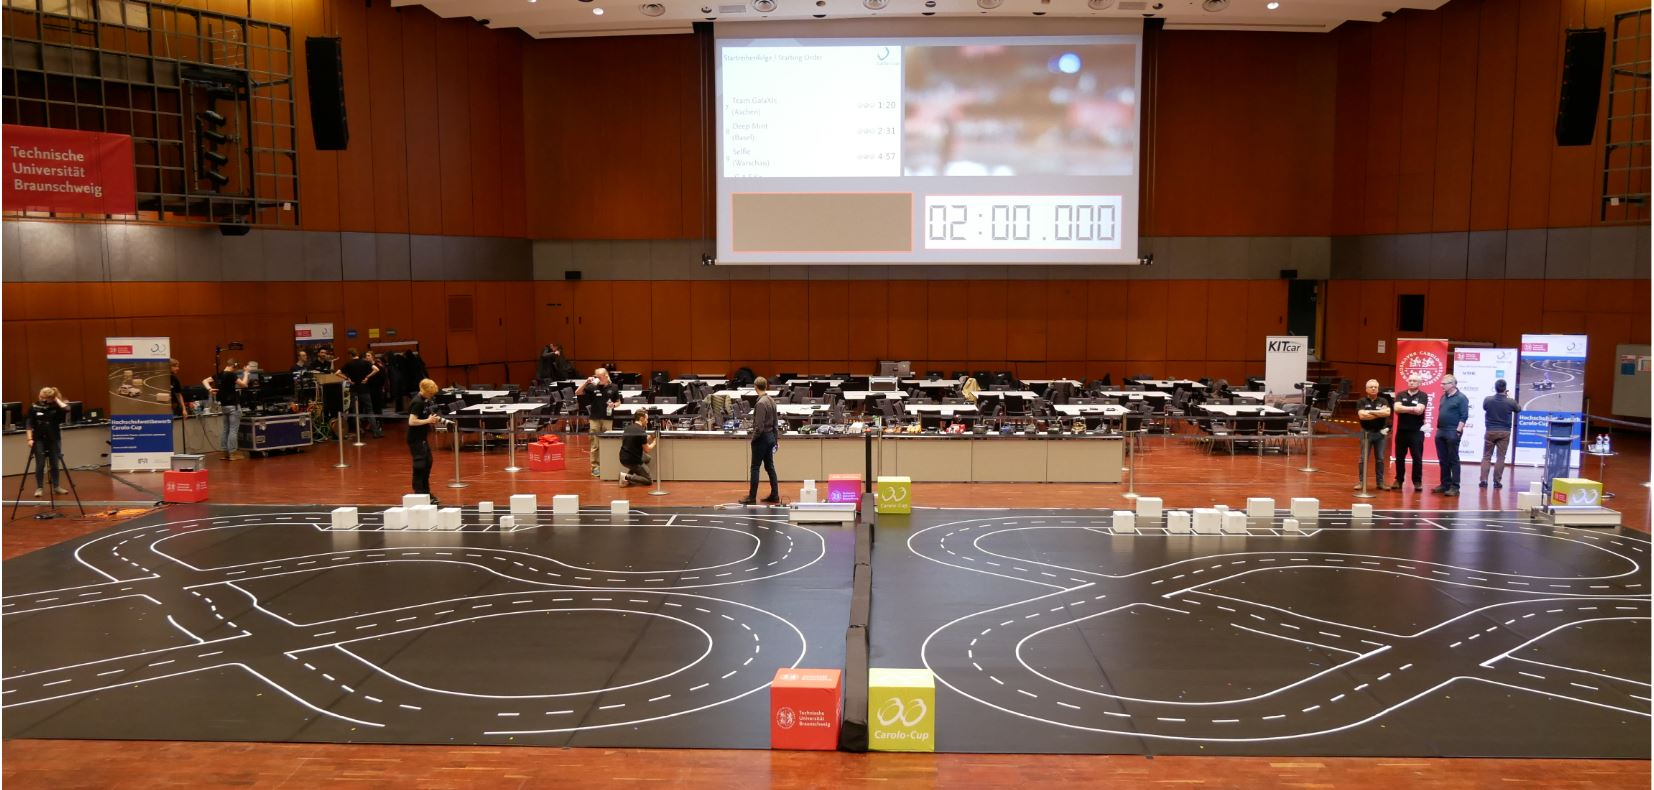
\includegraphics[width=\textwidth]{images/Einleitung/Carolocup.JPG}
  \caption[Strecke des Carolo-Cup 2020 an der TU Braunschweig]{Strecke des Carolo-Cup 2020 an der TU Braunschweig}
  \label{EIN:FOT}
\end{figure}
\FloatBarrier

\section{Zielsetzung}

Zur Zeit existieren verschiedene Ansätze, um die Software für autonome Fahrzeuge zu strukturieren. In dieser Arbeit wird eine Softwarearchitektur ausgewählt, mit der die Aufgabenstellung des Carolo-Cup 2020 erfüllt werden kann. Es wird festgelegt, wie der Datenfluss im Fahrzeug gestaltet werden soll und aus welchen Modulen das System bestehen soll. Die Architektur soll zudem möglichst leicht erweiterbar und nachvollziehbar sein.

Eine weitere wichtige Konzeptentscheidung ist die Wahl der Plattform für das autonome Fahrzeug. Es wird zwischen verschiedenen Betriebssystemen und Rechnersystemen abgewogen. Dabei wird beachtet, welche Umgebung die schnelle Erprobung neuer Softwarebestandteile erlaubt. Die Ausführung der Software soll dabei möglichst performant und unter Echtzeitbedingung erfolgen. Zudem wird die Verhaltenssteuerung des autonomen Fahrzeugs als Teil dieser Arbeit entwickelt. Dieser Teil der Software entscheidet, welches Manöver das Fahrzeug zu einem bestimmten Zeitpunkt durchführen soll. Dies kann beispielsweise die Einleitung eines Überholmanövers oder eines Parkvorgangs sein. Um Entscheidungen zu treffen, greift die Verhaltenssteuerung auf aufbereitete Sensorsignale zurück. Die Verhaltenssteuerung steuert zudem die Lichter des Fahrzeugs, um die Manöver und den Zustand des Fahrzeugs anzuzeigen. Zusätzlich soll die Verhaltenssteuerung Eingaben der Fernsteuerung und der Tasten am Fahrzeug verarbeiten. 

	%!TEX root = ../dokumentation.tex

\chapter{Stand der Technik}
\section{Regelkreis Fahrzeug}
In einem Fahrzeug, das nicht autonom fährt, übernimmt der Fahrer die Aufgabe, die richtige Spur und Geschwindigkeit zu halten. Der Fahrer tritt somit als Regler auf. Zu den Aufgaben des Fahrers gehören neben der direkten Regelung die Planung der Fahrt. Dies beinhaltet die Wahl der geeigneten Strecke. Beispielsweise entscheidet der Fahrer, ob er sein Ziel besser über die Autobahn oder Landstraßen erreichen kann. Auf der Strecke muss der Fahrer in der Lage sein, dynamisch auf Hindernisse wie beispielsweise Baustellen, Straßensperren und Kreuzungen reagieren \cite{MIT15}.

Die menschliche Informationsverarbeitung bietet sich offensichtlich für den Entwurf eines autonom fahrenden Systems an. Rasmussen unterteilt in \cite{RAS83} das Verhalten eines Menschen in drei verschiedene Ebenen. Dies ist in Abbildung \ref{RAS:INF} veranschaulicht. Unter Fertigkeiten ordnet Rasmussen stark automatisiertes Verhalten ein. Der Mensch muss hierbei nicht besonders aufmerksam sein. Aktionen die auf dieser Verhaltensebene durchgeführt werden als regelbasiertes Verhalten beschrieben. In Situationen die unbekannt sind, wird, nach Rasmussen, auf wissensbasierte Verhaltensweisen zurückgegriffen. Dieses Modell dient als Grundlage für viele weitere Theorien und kann für den Entwurf von Agenten für das autonome Fahren verwendet werden.
\FloatBarrier
\begin{figure}[h]
  \centering
  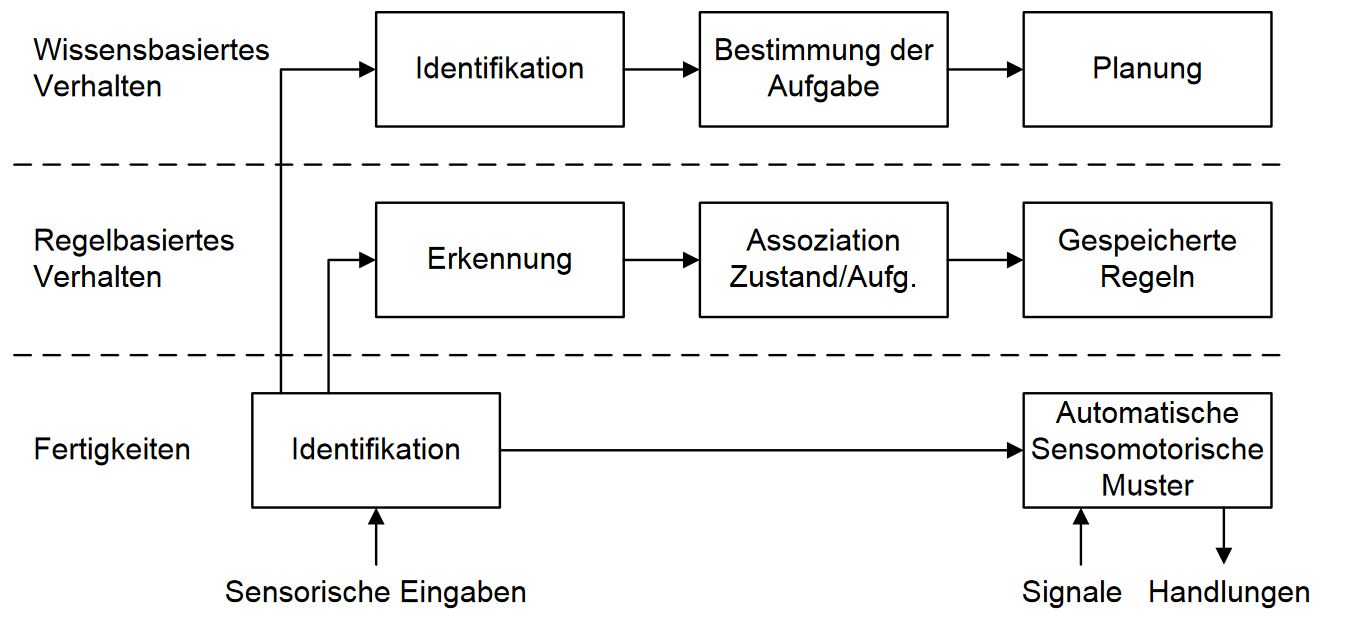
\includegraphics[width=0.9\textwidth]{images/stand_der_technik/Rasmussen.JPG}
  \caption[Informationsverarbeitung nach Rasmussen]{Informationsverarbeitung nach Rasmussen \cite{RAS83}}
  \label{RAS:INF}
\end{figure}
\FloatBarrier

\section{Das autonome Fahrzeug als kognitives System}
Nach \cite{TAS16} kann ein autonomes Fahrzeug genauso wie ein Mensch als kognitives System betrachtet werden. Dieses System lässt sich in drei Komponenten gliedern. Diese sind in Abbildung \ref{kog:sys} gezeigt. Das Perzeptions-Modul verarbeitet die Daten der Sensoren. Dazu gehören unter anderem die Lokalisierung des Fahrzeugs und die Erkennung von relevanten Objekten. Diese Informationen werden an das kognitive Entscheidungs System weitergeleitet. Dieses entscheidet und plant, welche Aktionen durchgeführt werden sollen. Die Durchführung der ausgewählten Aktion wird von der Komponente Aktion übernommen. Dieses regelt beziehungsweise steuert die Aktoren des Autonomen Fahrzeugs. Das gesamte Fahrzeug steht damit in einem Regelkreis mit der Umgebung.
\FloatBarrier
\begin{figure}[h]
  \centering
  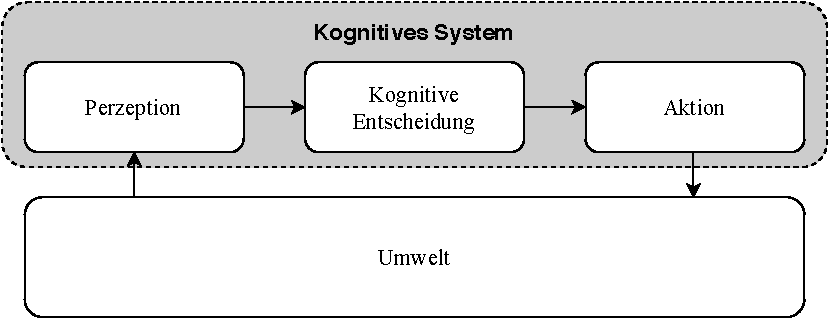
\includegraphics[width=0.8\textwidth]{images/stand_der_technik/kognitivesSystem.pdf}
  \caption[Aufbau eines kognitiven Systems]{Aufbau eines kognitiven Systems}
  \label{kog:sys}
\end{figure}
\FloatBarrier

\section{Bestehende Ansätze zur Strukturierung der Software für autonome Fahrzeuge}
Es bestehen unterschiedliche Ansätze, ein Software-System für autonome Fahrzeuge zu gestalten. Nach \cite{JUN14} unterscheiden sich grundsätzlich zwei verschiedene Ansätze. Zum einen die hierarchische Struktur und zum anderen die parallele Struktur. Zudem wird eine manöverbasierte Struktur vorgestellt.

\subsection{Hierarchische Struktur}
Hierarchische Strukturen bestehen aus Modulen die in verschiedenen Ebenen angeordnet sind. Auf jeder Ebene wird die Eingabe, die Mission, der nächsthöheren Ebene in Submissionen aufgeteilt und an die unterliegende Schicht weitergegeben.

Abbildung \ref{abb:hir} zeigt die Umsetzung einer solchen Struktur. Das Perzeptionssystem analysiert in Echtzeit die Eingaben von Lidar, Kamera und anderen Sensoren. Das Mission planning System generiert dabei einen Weg mit Zwischenzielen. Dabei wird die Ankunftszeit, benötigte  Manöver und die Distanz berücksichtigt. Das Behavior executive System fällt Entscheidungen über taktische Fahrmanöver wie Überholmanöver, Spurwechsel oder Interaktionen mit anderen Fahrzeugen. Im Motion planning Modul wird dann die endgültige Trajektorie errechnet. Dabei werden insbesondere der gewünschte  Lenkwinkel und die gewünschte Gaspedalstellung festgelegt.

Nach \cite{JUN14} ist ein Nachteil dieser Architektur, dass hierarchisch hoch oben angesiedelte Module nicht genügend Informationen haben und weiter unten angesiedelte Module nicht die Autorität die bereits getroffenen Entscheidungen zu redigieren.
\FloatBarrier
\begin{figure}[h]
  \centering
  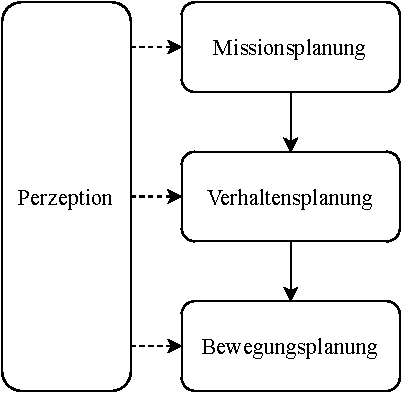
\includegraphics[width=0.5\textwidth]{images/stand_der_technik/hierarchische_struktur.pdf}
  \caption[Hierarchische Softwarestrukur f\"ur autonome Fahrzeuge]{Hierarchische Softwarestrukur f\"ur autonome Fahrzeuge nach \cite{JUN14}}
  \label{abb:hir}
\end{figure}
\FloatBarrier
\subsection{Parallele Struktur}
Die parallele Struktur verfolgt den Ansatz, verschiedene Module gleichzeitig auszuführen. In Abbildung \ref{par:str} ist dies gezeigt. Die Regler Module arbeiten unabhängig voneinander und verwenden zur Berechnung die Daten des Perzeptions Moduls. Oftmals sind dabei eigene Sensoren für jeden Regler vorgesehen. Der Vorteil ist hierbei, dass die Regler unabhängig voneinander ausgelegt und ausgetauscht werden können. Problematisch sind hierbei jedoch die Ausführung von sehr komplexen Fahrmanövern, da die Regler nicht aufeinander abgestimmt sind \cite{JUN14}. Zudem ist es oftmals nur schwer möglich, diese System zu erweitern, da dafür meist jedes Modul angepasst werden muss.
\FloatBarrier
\begin{figure}[t]
  \centering
  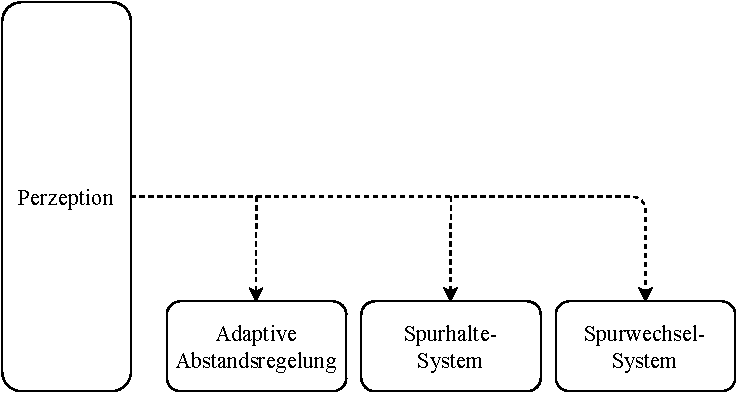
\includegraphics[width=\textwidth]{images/stand_der_technik/parallele_struktur.pdf}
  \caption[Parallele Softwarestruktur für autonome Fahrzeuge]{Parallele Softwarestruktur für autonome Fahrzeuge nach \cite{JUN14}}
  \label{par:str}
\end{figure}
\FloatBarrier

\subsection{Manöverbasierte Struktur}
In \cite{DUA20} wird eine manöverbasierte Softwarestruktur für eine autonomes Fahrzeug vorgestellt. Diese Softwarestruktur basiert auf neuronalen Netzwerken, die in Modulen ausgeführt werden. Jedes Modul ist für die Ausführung eines Manövers zuständig. Ein Manöver kann beispielsweise ein Spurwechsel, ein Einparkvorgang oder das Halten an einer Kreuzung sein. Diese Manöver werden jeweils vom zugehörigen Modul durchgeführt. Ein weiteres Modul entscheidet, welches Manöver im Moment durchgeführt werden soll. Das Fahrzeug führt zu jedem Zeitpunkt ein Manöver aus. Es handelt sich somit bei dieser Software-Struktur auch um eine hierarchische Struktur nach \cite{JUN14}.

In \cite{DUA20} wird beschrieben, dass beim Übergang zwischen Manövern Sprünge auf den Ausgangssignalen für die Aktoren im Fahrzeug entstehen können. Dies äußert sich als ruckartige Bewegung im Fahrzeug und kann besonders während dem Fahren gefährlich werden. Der Vorteil dieser Struktur ist insbesondere, dass die Module unabhängig voneinander entwickelt werden können. Zudem können die Module sehr leicht ausgetauscht werden. Darüber hinaus kann das Verhalten an komplexere Umgebungen angepasst werden, indem weitere Module für bestimmte Manöver hinzugefügt werden.

\FloatBarrier
\begin{figure}[h]
  \centering
  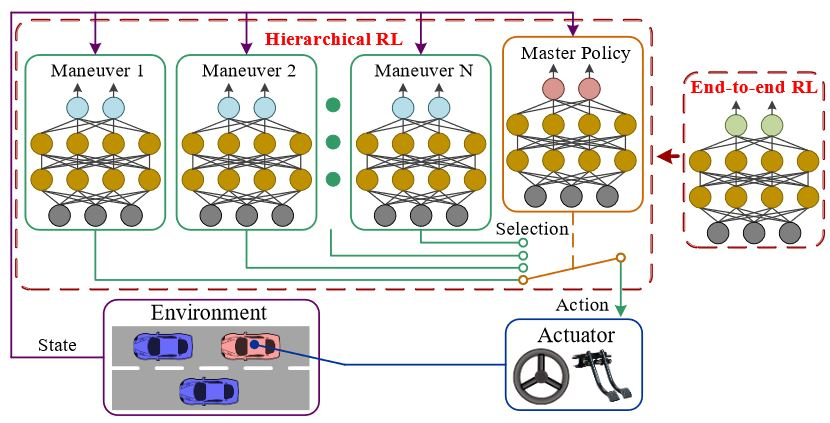
\includegraphics[width=\textwidth]{images/stand_der_technik/NN_SW_Structure.JPG}
  \caption[Manöverbasierte Softwarestruktur für autonome Robotor]{Manöverbasierte Struktur für autonome Robotor nach \cite{DUA20}}
  \label{NN:SW}
\end{figure}
\FloatBarrier

\section{Modellierung von Verhaltensweisen}
Die Informatik bietet verschiedene Möglichkeiten Verhaltensweisen zu modellieren. Diese sind im Bereich des autonomen Fahrens relevant, um die Verhaltenssteuerung der Fahrzeuge zu realisieren.

\subsection{Finite deterministische Zustandsautomaten}
Zustandsautomaten (kurz FSM) werden in der Informatik verwendet um Protokolle oder Verhaltensweisen zu beschreiben. Ein Zustandsautomat wird durch ein 5-Tupel $\mathcal{A} = (Q, \Sigma, \delta, q_0, F)$ definiert. Diese Bestandteile sind wie folgt definiert:
\begin{itemize}
 \item $Q$ einer Menge von Zuständen $q_i$
 \item $\Sigma$ einem Eingabealphabet
 \item $\delta(q, a)=q': Q \times \Sigma \rightarrow Q$ eine Transitions- oder Übergangsfunktion, die einen Zustand in einen anderen überführt
 \item $q_0 \in Q$ dem Startzustand
 \item $F \subset Q$ der Endzustandsmenge
\end{itemize}

Die Wartung von Zustandsautomaten ist aufwändig, wenn Zustände oft hinzugefügt oder entfernt werden sollen. Es wird dann notwendig eine große Anzahl von Übergängen zwischen Zuständen einzufügen oder zu löschen. Dabei besteht die Möglichkeit, dass Fehler passieren die übersehen werden. Besonders große Zustandsautomaten sind oftmals schlecht zu überblicken. 

\subsection{Hierarchische Zustandsautomaten}
Das Modell der Hierarchischen Zustandsautomaten (engl. Hierarchical State Machines, kurz HFSM) ist ein erweitertes Model der FSM. HFSM erlauben die Schachtelung von Zuständen und somit Subautomaten und Subzustände zu bilden.  

In einem HFSM existiert immer ein Top-Zustand. Dieser ist der oberste Zustand im Modell. Anderen Zustände können Subzustände dieses Top-Zustands sein. Zustände können beliebig tief verschachteltet werden. Wenn ein Subzustand aktiv ist bedeutet dies, dass alle Top-Zustände auch aktiv sind. Der Zustand, der direkt über dem relevanten Subzustand liegt, wird Super-Zustand genannt. 
HFSM eignen sich besonders für die Modellierung komplexer Verhaltensweisen. Ein einfacher HFSM ist in Abbildung \ref{HFS:PLC} gezeigt. Dieser HFSM besteht aus zwei Super-Zuständen mit jeweils zwei Sub-Zuständen.
\FloatBarrier
\begin{figure}[h]
  \centering
  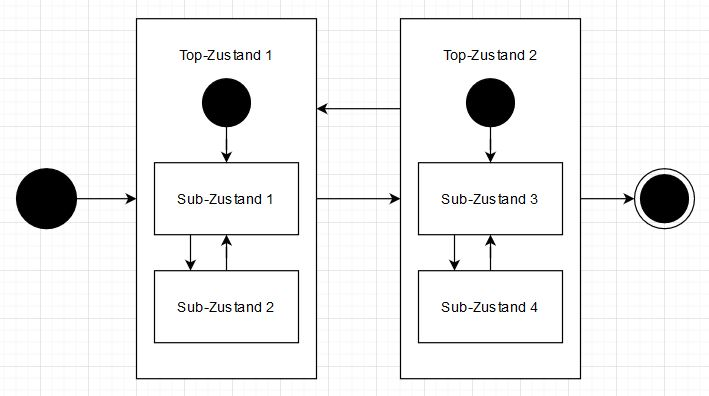
\includegraphics[width=0.7\textwidth]{images/stand_der_technik/HFSM_Plazebo.JPG}
  \caption[Finiter endlicher Zustandsautomat]{Finiter endlicher Zustandsautomat}
  \label{HFS:PLC}
\end{figure}
\FloatBarrier

\subsection{Verhaltensbäume}
Verhaltensbäume werden insbesondere in der Computerspiele-Industrie verwendet, um das Verhalten von Agenten zu beschreiben. Das Grundkonzept beruht darauf, dass elementare Aktionen auf denen die Verhaltensweise basiert, baumartig strukturiert sind.

Die Ausführung eines Verhaltensbaums erlaubt keine Speicherung von Zuständen. Dies gestaltet die Ausführung von Sequenzen sehr schwierig die länger als die Zwischenzeit zwischen den einzelnen "Ticks" dauert. Daraus  resultiert insbesondere ein Problem wenn eine bestimmte Sequenz über mehrere \"Ticks\" ausgeführt werden soll. Es kann somit passieren, dass die Ausführung einer Sequenz unterbrochen wird, obwohl eine andere Aktion im Moment ausgeführt werden soll. In \cite{KLC15} wird ein Ansatz, vorgestellt einen Verhaltensbaum mit einem Speicher für Zustände zu realisieren vorgestellt. Dabei geht jedoch auch ein Teil die Übersichtlichkeit des Baums verloren. Bei sehr großen Verhaltensbäumen können Laufzeitprobleme auftreten, da der Baum immer von der Wurzel durchlaufen wird. 

\subsection{Neuronale Netze}
Das Konzept von künstlicher Intelligenz mit neuronalen Netzen ist am menschlichen Gehirn orientiert. Besonders in den letzten Jahren konnten mithilfe von neuronalen Netze Durchbrüche in der Bilderkennung [XYZ] und der Robotik [XYZ] erreicht worden. Grigorescu et. al. beschreiben in \cite{GRI19}, dass künstliche Intelligenz durch neuronale Netze zur Verhaltenssteuerung in autonomen Fahrzeugen bereits in Projekten wie beispielsweise der DARPA challenge 2017 erfolgreich eingesetzt wurden. In \cite{MIR18} wird beispielsweise ein Verfahren vorgestellt, das es erlaubt mithilfe eines neuronalen Netzes zu entscheiden, ob ein Überholvorgang eingeleitet werden kann. Hier wird gezeigt, dass es möglich ist, mit diesem Ansatz in Fahrzeugen Entscheidungen autonom zu treffen. 

Ein neuronales Netz wird analog zu einem Graphen über eine Menge an Kanten und Knoten also Neuronen und Verbindungen definiert. Jede Verbindung hat ein Gewicht und jedes Neuron einen Bias. Zusätzlich wird eine Aktivierungsfunktion für jedes Neuron definiert \cite{CIT11}.

Die Netzwerke müssen vor dem Einsatz angelernt werden. Dazu ist die Verwendung einer Simulationsumgebung notwendig, da so Testfahrten sicher durchgeführt werden können. Zusätzlich können Tests so automatisiert durchgeführt werden. Dies erlaubt es das Netzwerk schnell anzupassen, da die meisten Simulationen die Realität nicht genügend genau abbilden. Daher kann es passieren, dass die in der Simulation erprobten neuronalen Netze nicht direkt auf eine reale Umgebung anwendbar sind \cite{GRI19}. Zusätzlich stellt die Realisierung einer detailgetreuen Simulationsumgebung meist einen sehr hohen Arbeitsaufwand dar. Aufgrund der hohen Komplexität größerer neuronaler Netze ist die Verhaltensweise oftmals nur schwer nachvollziehbar. Besonders das zuvor beschriebene eigenständige Erlernen bestimmter typischer Verhaltensweisen kann zu Problemen führen. Um die Sicherheit zu gewährleisten, sollten nach \cite{GRI19} zusätzliche Sicherheitsmaßnahmen wie beispielsweise Watchdogs etc. erwogen werden. Damit soll das Fahrzeug im Zweifel in einen sicheren Zustand überführt werden. Ein Nachweis über die funktionale Sicherheit des Systems müsste daher durch Statistiken, die über viele Fahrstunden erstellt werden. 

\section{Betriebssysteme}
Autonom fahrende Fahrzeuge verfügen oftmals über ein Zentralsteuergerät zur Ausführung komplexer Aufgaben. Dieses Zentralsteuergerät verfügt zumeist über ein Betriebssystem. Zu den Aufgaben des Betriebssystems gehört die Verteilung der Rechenzeit unter den einzelnen Prozessen, die Anbindung von Peripheriegeräten und die Bereitstellung von grundlegenden Diensten. Die Alternative zur Verwendung eine Betriebssystems ist der Aufbau eines monolithischen Softwaresystems. Je nachdem wie komplex und groß das Softwaresystem wird, kann dies sehr kompliziert zu warten und zu erweitern werden.

\subsection{Robot Operating System}
Das Robot Operating System (kurz ROS) ist ein open-source Software-Framework, das die Entwicklung komplexer modularer Softwaresysteme für Roboter unterstützt. ROS benötigt zur Ausführung zusätzlich ein zugrundeliegendes Linux Betriebssystem. Applikationen, die auf ROS aufsetzen, können in C++ oder Python geschrieben werden. ROS übernimmt die Kommunikation zwischen einzelnen Softwaremodulen und bietet eine Vielzahl an bestehenden Erweiterungen an. Anwendungen können mithilfe von ROS auf verschiedene Rechner aufgeteilt werden \cite{AND16}.

Systeme, die auf dem Robot Operating Systems basieren, bestehen meist aus mehreren einzelnen Modulen, sogenannte \textit{Nodes} oder \textit{Nodelets}. Diese Module können auf verschiedenen Wegen miteinander kommunizieren. Die Kommunikation wird von einem Master Server verwaltet.  
In Abbildung \ref{ros:str} ist zu sehen, dass dieser Server auch \textit{Nodes} ausführen kann. Weitere Slave Server können ihre \textit{Nodes} beim Master registrieren und werden somit serverübergreifend erreichbar. Zur Kommunikation zwischen den Servern wird das TCP oder UDP Protokoll verwendet.
\FloatBarrier
\begin{figure}[h]
  \centering
  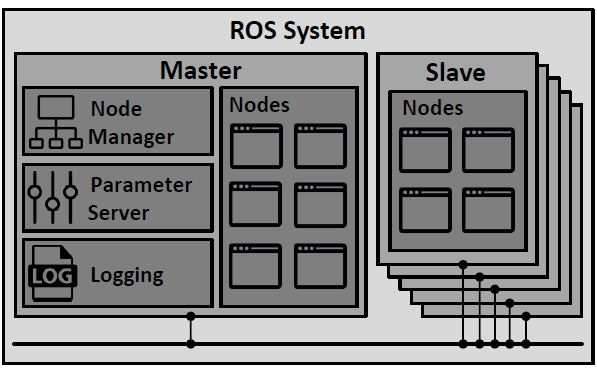
\includegraphics[width=\textwidth]{images/stand_der_technik/ROS_AS.JPG}
  \caption[Struktur des Robot Operating System]{Struktur des Robot Operating System}
  \label{ros:str}
\end{figure}
\FloatBarrier
Nachrichtentypen können ähnlich wie Objekte in C++ in ROS beschrieben werden. Darüber hinaus stehen dem Anwender einige Grundtypen zur Verfügung. Diese Grundtypen decken sich mit weitestgehend den Datentypen in C++ \cite{AND16}.

Die Kommunikation zwischen den \textit{Nodes} erfolgt über das Publish/Subscribe-Prinzip. Dies bedeutet, dass Nodes sogenannte Topics mit einem bestimmten Nachrichtentyp beim Master registrieren können. Alle angebundenen Nodes können daraufhin diesem Topic subscriben und erhalten dann immer die zuletzt gesendete Nachricht auf diesem bestimmten Topic. Es können auch mehr als ein Node auf einem bestimmten Topic publischen.

\subsection{Automotive Data and Time-Triggered Framework}
Das Automotive Data and Time-Triggered Framework (ADTF) ist eine propietäre Software die von der Firma Elektrobit vermarktet wird. Es ist ein Echtzeitsystem und wird zur Entwicklung von sogenannten Advanced Driver Assistance Systemen (ADAS) verwendet. Die Software unterstützt das synchrone und asynchrone Verarbeiten von Daten. Es ermöglicht die Erprobung der Software in Simulationsumgebung und die Programmierung von Softwarebestandteilen in C und C++. Darüber hinaus können über Toolboxen Programmierumgebungen wie Matlab/Simulink angebunden werden. Da ADTF ein professionell lizenziertes Produkt ist wird es hauptsächlich von Unternehmen verwendet. Die Community des ADTF ist daher nur sehr klein \cite{AND16}.

\section{Aufbau des Fahrzeugs der DHBW Smart Rollerz}
Das Fahrzeug verfügt über einen Elektromotor, der über ein Getriebe mit allen Rädern verbunden ist. Darüber hinaus wird ein Servomotor verwendet, um die Vorderräder zu lenken. Zusätzlich sind Lichter am Fahrzeug angebracht. Diese dienen dazu, Manöver korrekt anzuzeigen und die Verwendung der Fernbedienung durch eine leuchtende blaue LED zu signalisieren. In Abbildung \ref{sen:zeg} ist das aufgebaute autonom fahrende Fahrzeug zu sehen.

\FloatBarrier
\begin{figure}[h]
  \centering
  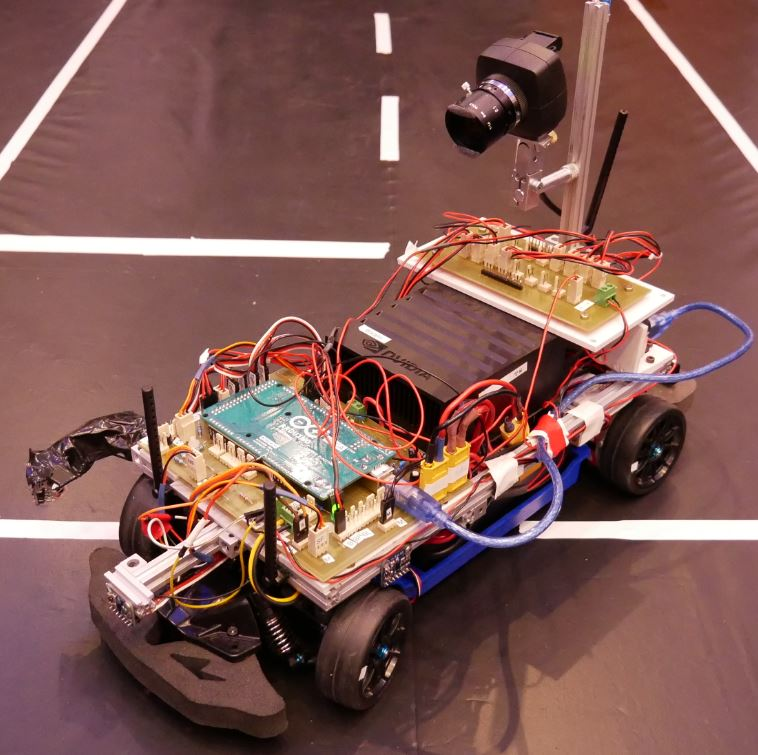
\includegraphics[width=0.5\textwidth]{images/stand_der_technik/SR_Fahrzeug.JPG}
  \caption[Fahrzeug der DHBW Smart Rollerz]{Fahrzeug der DHBW Smart Rollerz}
  \label{sen:zeg}
\end{figure}
\FloatBarrier

Das Fahrzeug verfügt über verschiedene Sensoren, um die Umgebung des Fahrzeugs zu erkennen. Ein Überblick über die angebrachten Sensoren gibt Abbildung \ref{sen:auf}. Die Kamera wird 30 Zentimeter über dem Fahrzeug montiert und ist nach vorne gerichtet. Dies soll es ermöglichen, die Spuren der Fahrbahn, Kreuzungen, Parkplätze und die Startlinie zu erkennen. Zusätzlich sind drei Distanzsensoren am Fahrzeug angebracht. Sie haben einen Messbereich von etwa 3 Zentimetern zu einem Meter. Der nach vorne gerichtete Distanzsensor soll vorrausfahrende Fahrzeuge erkennen. Um Vorfahrtssituationen zu erkennen wird ein schräg nach vorne gerichteter Sensor verwendet. Der seitlich angebrachte Distanzsensor kommt beim Erkennen und Vermessen von Parklücken als auch bei Überholvorgängen zum Einsatz. Zur Bestimmung der Geschwindigkeit verfügt das Fahrzeug zudem über einen Drehzahlsensor und einen Beschleunigungsmesser. Der Beschleunigungsmesser soll es ermöglichen, die Geschwindigkeit genauer zu ermitteln und die Kurvenbeschleunigung für die Regelung zu messen.

\FloatBarrier
\begin{figure}[h]
  \centering
  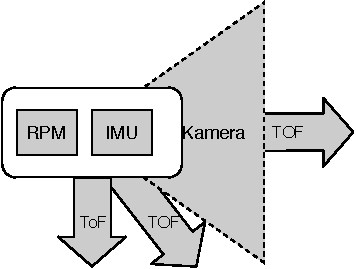
\includegraphics[width=0.3\textwidth]{images/stand_der_technik/Sensoren.pdf}
  \caption[Sensorik des aufgebauten Fahrzeugs]{Sensorik des aufgebauten Fahrzeugs}
  \label{sen:auf}
\end{figure}
\FloatBarrier
	%!TEX root = ../dokumentation.tex
\chapter{Aufbau und Struktur des Softwaresystems}

\section{Konzept des Softwaresystems}
Für die Softwarestruktur wird ein hierarchischer Struktur nach \cite{}
In Abbildung \ref{SOF:STR} ist die Struktur und insbesondere der Datenfluss zwischen den einzelnen Modulen gezeigt.

\FloatBarrier
\begin{figure}[t]
  \centering
  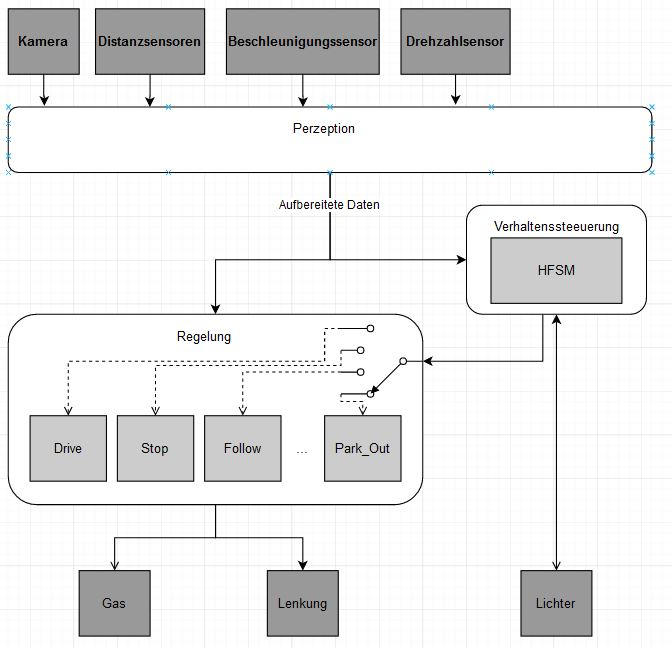
\includegraphics[width=0.5\textwidth]{images/Verhaltenssteuerung/SW_Structure.JPG}
  \caption{Softwarestruktur}
  \label{SOF:STR}
\end{figure}
\FloatBarrier

\section{Implementierung des Softwaresystems}
\subsection{Rechnersystem}

\subsection{Betriebssystem}
Für den Betrieb 
\subsection{Aufteilung der Software in Module}
\subsection{Kommunikation zwischen den Modulen}

\section{Implementierung der Verhaltenssteuerung}




\subsection{Datenaufbereitung}
Um die Daten für die Entscheidung über Zustandsübergänge zu erhalten müssen die Sensorwerte aus dem Perzeptionsmodul ausgelesen und verarbeitet werden. Dies wird in einem dafür vorgesehen Modul durchgeführt. Direkt verwendbare Daten aus dem Perzeptionsmodul werden nicht über das Datenaufbereitungsmodul an die Verhaltenssteuerung weitergegeben, sondern direkt in der Verhaltenssteuerung verwendet. In der untenstehenden sind alle Übergangsbedingungen gelistet und dargestellt ob diese im Datenaufbereitungsmodul generiert werden. 

Zeit abgelaufen         -> Datenaufbereitung
Fernbedienung aktiviert -> direkt
Taster Obstacle Evasion -> direkt
Taster Free Drive       -> direkt


\section{Grafische Oberfläche}
Die Grafische Oberfläche soll es ermöglichen währendem das Fahrzeug autonom fährt einzusehen in welchem Zustand sich das Fahrzeug befindet. Dies ermöglicht schnelle Rückschlüsse beim Testen und ermöglicht somit eine effiziente Entwicklung.
\subsection{Fahrtbeginn}
\subsection{Datenauswertung nach der Fahrt}






	%!TEX root = ../dokumentation.tex

\chapter{Zusammenfassung}
\section{Limitierungen}
\section{Ausblick}
	\clearpage


	% Quellcodeverzeichnis
	%\cleardoublepage
	%\phantomsection \label{listoflist}
	%\addcontentsline{toc}{chapter}{Listings}
	%\lstlistoflistings
    \renewcommand{\thepage}{\Roman{page}}
	\setcounter{page}{13}
	%!TEX root = ../dokumentation.tex
\chapter{Anhang}
\appendix

	% Literaturverzeichnis
	\cleardoublepage
	\phantomsection \label{listoflit}
	\addcontentsline{toc}{chapter}{Literaturverzeichnis}
	
	%Bib style
	%\bibliographystyle{agsm} %Havard
	%\bibliographystyle{amsplain} %Durchnummeriert
	%\bibliographystyle{amsalpha} %Kürzel für Autor und Jahr
	%see more: http://amath.colorado.edu/documentation/LaTeX/reference/faq/bibstyles.pdf

	\printbibliography[title=Literaturverzeichnis]

	% Glossar
	\printglossary[style=altlist,title=Glossar]
\end{document}
